\documentclass[]{beamer}

\usepackage{lipsum}
\usepackage{pgfpages}
\usepackage{graphics}

\graphicspath{{img/}}

\mode<handout>{%
%	\setbeameroption{show notes}
}

\usetheme{AnnArbor}
\usecolortheme{beaver}

\AtBeginSection[]
{
	\begin{frame}
		\frametitle{Inhoudsopgave}
		\tableofcontents[currentsection]
	\end{frame}
}


\begin{document}
	\title[Actieherkenning met de Kinect sensor]{Intuïtive mens-machineinterface met live actieherkenning }
	\author[Bert De Saffel]{
				\begin{tabular}{rcr}
				prof. dr. ir. Peter Veelaert &\&& prof. dr. ir. Wilfried Philips \\
				ing. Sanne Roegiers &\&& ing. Dimitri van Cauwelaert
				\end{tabular}
	}
	
	\subtitle{Master of Science in de industriële wetenschappen: informatica \\ \vspace{0.2cm} Bert De Saffel}
	\date{04 april 2019}
	\frame{\titlepage}
	
	\section{Vorige week}
	\frametitle{Vorige week}
	\begin{frame}
		\begin{itemize}
			\item Kleurenbeelden opslaan
			\item Gelabelde dataset
			\begin{itemize}
				\item Drie personen
				\item Elke persoon voert vijf maal elke actie uit
			\end{itemize}
			\item Normaliseren skeletjoints
			\begin{itemize}
				\item Pelvis als centrum
				\item Elke andere joint is relatief t.o.v. het centrum 
			\end{itemize}
		\end{itemize}
	\end{frame}
	
	\section{Context}
	\begin{frame}
		\begin{itemize}
			\item Real-time actieherkenning
			\item Met de Kinect Sensor
			\begin{itemize}
				\item Genereert skelet via dieptebeelden
			\end{itemize}
		\end{itemize}
		\begin{figure}
			\centering
			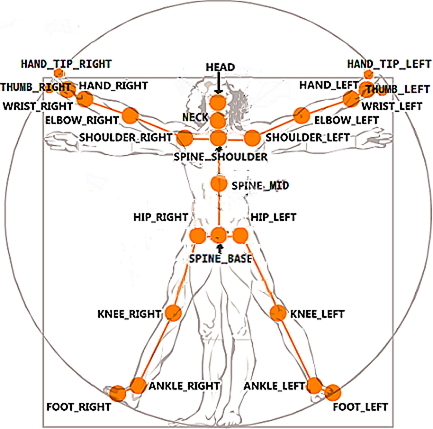
\includegraphics[width=0.4\textwidth]{skeleton}
		\end{figure}
	\end{frame}

	\section{Probleemstelling}
	\begin{frame}
		\frametitle{Probleemstelling}
		\begin{itemize}
			\item Invariant zijn van de features onafhankelijk van o.a.:
			\begin{itemize}
				\item verschillen in lichaamsbouw (kind of volwassen)
				\item actie-uitvoering
				\item camerahoek
				\item snelheid (trage of snelle actie)
			\end{itemize}
		\end{itemize}
		\begin{figure}
			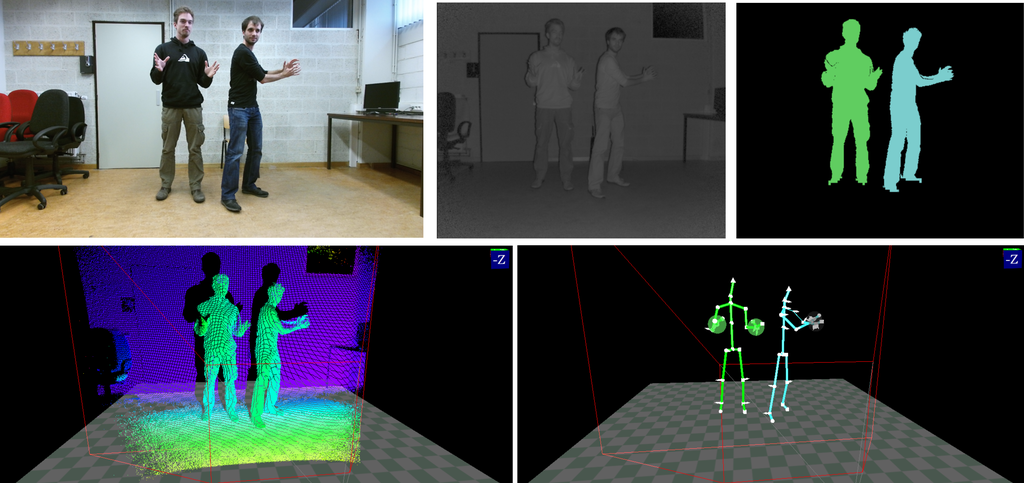
\includegraphics[width=0.7\linewidth]{sensoren}
		\end{figure}
	\end{frame}
	\begin{frame}
			\frametitle{Probleemstelling}
	\begin{itemize}
		\item Invariant zijn van de features onafhankelijk van o.a.:
		\begin{itemize}
			\item verschillen in lichaamsbouw (kind of volwassen)
			\item actie-uitvoering
			\item camerahoek
			\item snelheid (trage of snelle actie)
		\end{itemize}
	\end{itemize}
	\begin{figure}
		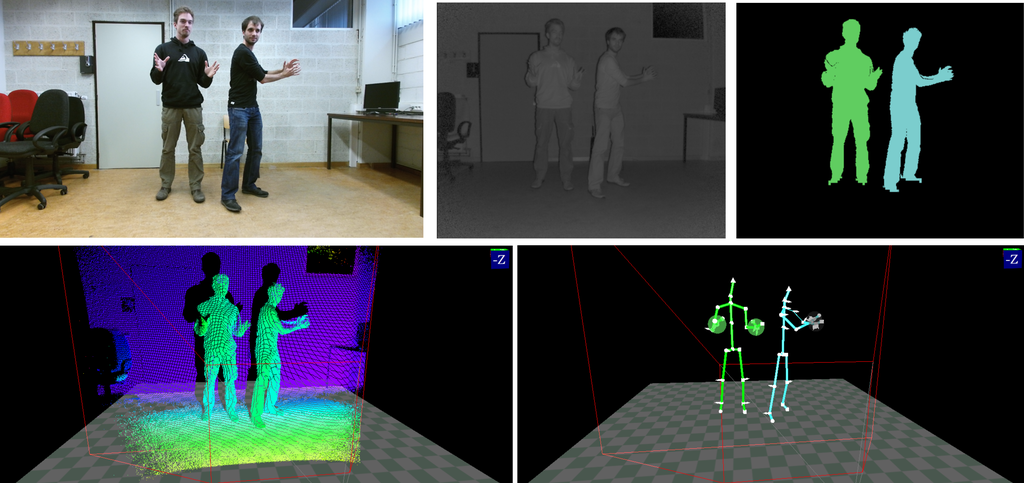
\includegraphics[width=0.7\linewidth]{sensoren}
	\end{figure}
	\end{frame}

	\section{Realisatie}

	\begin{frame}
		\frametitle{Realisatie}
		\begin{itemize}
			\item Eigen dataset gemaakt
			\begin{itemize}
				\item 3 personen
				\item 9 acties
				\item Elke actie 5 keer
			\end{itemize}
		\end{itemize}
	\end{frame}


	\begin{frame}
		\begin{center}
			\Huge Vragen, opmerkingen, ...?
		\end{center}
	\end{frame}
\end{document}